\documentclass{beamer}

\newcommand{\delim}{\line(1,0){290}}
\newcommand{\norma}[1]{\Vert #1 \Vert_2}
\newcommand{\modulo}[1]{\vert #1 \vert}
\newcommand{\prodint}[2]{\langle #1,#2 \rangle}
\newcommand{\barrav}[1]{\line(0,1){#1}}
\newcommand{\ssiz}{\scriptsize}
\newcommand{\xsol}{\overline{x}}
\newcommand{\xmu}{x(\mu)}

%\setbeamercolor{cordotitulo}{bg=green!30!black,fg=white}
\useinnertheme{rounded}
\setbeamercolor{structure}{fg=teal!80!blue}
%\useoutertheme{smoothbars}
%\useoutertheme{shadow}
\useoutertheme[height=1 cm,width=1.5 cm]{sidebar}
%\usecolortheme{crane}
%\setbeamerfont{frametitle}{shape=\itshape}
\setbeamercolor{palette primary}{bg=teal!80!blue,fg=white}
\setbeamercolor{palette secondary}{bg=white,fg=white} %cor do logo
\setbeamercolor{palette tertiary}{bg=blue!70!black,fg=white}
\setbeamercolor{palette quaternary}{bg=white,fg=teal!80!blue}
\setbeamercolor{sidebar}{bg=teal!80!blue}
%\setbeamercolor{palette sidebar primary}{bg=red,fg=black}
%\setbeamercolor{palette sidebar secondary}{bg=red,fg=black}
\setbeamercolor{palette sidebar tertiary}{fg=white} %Autor no sidebar
\setbeamercolor{palette sidebar quaternary}{fg=white} %Titulo no sidebar
\setbeamercolor{section in sidebar}{fg=teal!80!blue,bg=white} %A cor naum
\setbeamercolor{subsection in sidebar}{fg=teal!80!blue,bg=white} %A cor naum
%ativa parece ser uma media das duas
%\setbeamercolor{section in sidebar current}{fg=red}
\setbeamercolor{frametitle}{fg=white,bg=teal!80!blue} %mudar
%fg aqui
\setbeamercolor{title}{bg=teal!80!blue,fg=white}
\setbeamerfont{title}{series=\bf}
\setbeamercolor{author}{bg=teal!80!blue,fg=white}
\setbeamerfont{author}{series=\bf}
\setbeamercolor{normal text}{bg=white,fg=teal!50!black}
\logo{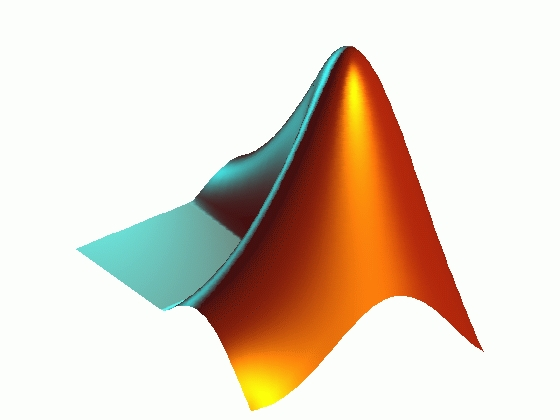
\includegraphics[scale=0.06]{matlab_logo.jpg}}

\title{Introdu\c{c}\~ao ao MatLab \\ Aula 7}
\author{Abel Siqueira \\ Kally Chung}
\date{}

\begin{document}

\frame{\titlepage}

\section[Gr\'aficos 3D]{}

\begin{frame}
\frametitle{Gr\'aficos 3D}

\begin{itemize}
 \item<1-> O Matlab permite criar gr\'aficos tridimensionais de curvas e de
superf\'icies.
 \item<2-> O gr\'afico de curvas \'e simplesmente uma extens\~ao do comando
{\tt plot}.
 \item<3-> Al\'em desse gr\'aficos tridimensionais, podemos criar tamb\'em
gr\'aficos de curvas de n\'ivel.
\end{itemize}

\end{frame}

\subsection[Fun\c{c}\~ao plot3]{}

\begin{frame}[fragile]
\frametitle{Fun\c{c}\~ao {\tt plot3}}
A fun\c{c}\~ao {\tt plot3} cria gr\'aficos de curvas. Ele faz como o comando
{\tt plot}, simplesmente tendo uma vari\'avel a mais, referente ao eixoz.

Exemplo 1:
{\scriptsize
\begin{verbatim}
>> t = linspace(0,2*pi,100);
>> plot3(sin(t),cos(t),t)
\end{verbatim}}
\pause
Esse c\'odigo gera o gr\'afico
\begin{center}
\includegraphics[scale=0.3]{aula7ex1.jpg}
\end{center}
\end{frame}

\begin{frame}[fragile]
\frametitle{Fun\c{c}\~ao {\tt plot3}}
A fun\c{c}\~ao {\tt plot3} tamb\'em aceita muitos dos comandos da fun\c{c}\~ao
{\tt plot}.

Exemplo 2:
{\scriptsize
\begin{verbatim}
>> t = linspace(0,2*pi,30);
>> plot3(sin(t),cos(t),t,`k:');
>> hold on
>> plot3(sin(t),cos(t),t+pi/3,`r--');
>> plot3(sin(t),cos(t),t+2*pi/3,`g-.');
\end{verbatim}}
\pause
Esse c\'odigo gera o gr\'afico
\begin{center}
\includegraphics[scale=0.3]{aula7ex2.jpg}
\end{center}
\end{frame}

\subsection[Superf\'icies]{}

\begin{frame}[fragile]
\frametitle{Superf\'icies}
\begin{itemize}
 \item<1-> Dadas tr\^es matrizes de mesma dimens\~ao X, Y e Z, o Matlab ir\'a
relacion\'a-las nessa ordem com as tr\^es dimens\~oes x, y e z.
 \item<2-> As fun\c{c}\~oes para plotar os gr\'aficos ir\~ao considerar os
elementos de posi\c{c}\~oes iguais e formar uma tripla ordenada, que ser\'a um
ponto que pertence ao gr\'afico.
 \item<3-> Dados dois vetores x e y, pode-se criar as matrizes X e Y
correspondentes usando {\tt [X,Y] = meshgrid(x,y)}.
 \item<4-> Normalmente, se a fun\c{c}\~ao $f$ \'e complicada, \'e necess\'ario
fazer loops relacionando cada elemento i,j de Z com os elementos x(i) e y(j),
fazendo {\tt Z(i,j) = $f$(x(i),y(j))}.
 \item<5-> Para fun\c{c}\~oes f\'aceis pode-se usar diretamente as matrizes X e
Y para montar Z. Por exemplo, para $f(x,y) = xy$, fazemos {\tt Z = X.*Y}.
\end{itemize}

\end{frame}

\begin{frame}[fragile]
\frametitle{Fun\c{c}\~ao {\tt mesh}}
A fun\c{c}\~ao {\tt mesh} plota o gr\'afico dado conectando os pontos
adjacentes, formando um esp\'ecie de rede.

Exemplo 3:
{\scriptsize
\begin{verbatim}
>> x = linspace(-5,5,30); y = x;
>> [X,Y] = meshgrid(x,y);
>> Z = X.^2-Y.^2;
>> mesh(X,Y,Z);
\end{verbatim}}
\pause
Esse c\'odigo gera o gr\'afico
\begin{center}
\includegraphics[scale=0.3]{aula7ex3.jpg}
\end{center}
\end{frame}

\begin{frame}[fragile]
\frametitle{Op\c{c}\~oes do {\tt mesh}}
\begin{itemize}
\item<1-> \'E poss\'ivel deixar o gr\'afico opaco ou transparente utilizando os
comandos {\tt hidden on} e {\tt hidden off} respectivamente.
\item<2-> O comando {\tt meshc} faz o mesmo que o {\tt mesh}, mas inclui curvas
de n\'ivel abaixo do gr\'afico.
\item<3-> O comando {\tt meshz} faz o mesmo que o {\tt mesh}, mas com um plano
no n\'ivel zero.
\item<4-> O comando {\tt waterfall} \'e semelhante ao {\tt mesh}, mas plota
apenas as linhas na dire\c{c}\~ao x.
\end{itemize}
\end{frame}

\begin{frame}[fragile]
\frametitle{Fun\c{c}\~ao {\tt surf}}
A fun\c{c}\~ao {\tt surf} \'e semelhante \'a fun\c{c}\~ao {\tt mesh}, por\'em
ele preenche e pinta o espa\c{c}o entre as linhas.

Exemplo 4:
{\scriptsize
\begin{verbatim}
>> x = linspace(-5,5,30); y = x;
>> [X,Y] = meshgrid(x,y);
>> Z = X.^2-Y.^2;
>> surf(X,Y,Z);
\end{verbatim}}
\pause
Esse c\'odigo gera o gr\'afico
\begin{center}
\includegraphics[scale=0.3]{aula7ex4.jpg}
\end{center}
\end{frame}

\begin{frame}[fragile]
\frametitle{Op\c{c}\~oes do {\tt surf}}

\begin{itemize}
\item<1-> Para deixar o gr\'afico liso, utilizamos {\tt shading flat}.
\item<2-> Para interpolar a pintura entre os espa\c{c}oes, utilizamos {\tt
shading interp}.
\item<3-> O comando {\tt surfc} faz o mesmo que o {\tt surf}, mas adiciona
curvas de n\'ivel abaixo do gr\'afico.
\item<4-> O comando {\tt surfl} faz o mesmo que o {\tt surf}, mas simulando a
ilumina\c{c}\~ao do objeto.
\item<5-> O comando {\tt surfnorm} faz o mesmo que o {\tt surf}, mas adiciona
vetores normais no gr\'afico.
\end{itemize}
\end{frame}

\subsection[Curvas de N\'ivel]{}

\begin{frame}[fragile]
\frametitle{Fun\c{c}\~ao {\tt contour}}
A fun\c{c}\~ao {\tt contour} plota uma quantidade dada de curvas de n\'ivel da
fun\c{c}\~ao dada. O comando {\tt colorbar} mostra a legenda de valores.

Exemplo 5:
{\scriptsize
\begin{verbatim}
>> x = linspace(-5,5,30); y = x;
>> [X,Y] = meshgrid(x,y);
>> Z = X.^2-Y.^2;
>> contour(X,Y,Z,30)
>> colorbar
\end{verbatim}}
\pause
Esse c\'odigo gera o gr\'afico
\begin{center}
\includegraphics[scale=0.25]{aula7ex5.jpg}
\end{center}
\end{frame}

\begin{frame}[fragile]
\frametitle{Fun\c{c}\~ao {\tt contour3}}
A fun\c{c}\~ao {\tt contour3} plota uma quantidade dada de curvas de n\'ivel da
fun\c{c}\~ao dada, em tr\^es dimens\~oes.

Exemplo 6:
{\scriptsize
\begin{verbatim}
>> x = linspace(-5,5,30); y = x;
>> [X,Y] = meshgrid(x,y);
>> Z = X.^2-Y.^2;
>> contour3(X,Y,Z,30)
\end{verbatim}}
\pause
Esse c\'odigo gera o gr\'afico
\begin{center}
\includegraphics[scale=0.25]{aula7ex6.jpg}
\end{center}
\end{frame}

\begin{frame}[fragile]
\frametitle{Fun\c{c}\~ao {\tt pcolor}}
A fun\c{c}\~ao {\tt pcolor} cria um quadriculado e pinta cada quadrado de acordo com o valor da fun\c{c}\~ao. Usando {\tt shading interp} obtemos uma suaviza\c{c}\~ao das cores.

Exemplo 7:
{\scriptsize
\begin{verbatim}
>> x = linspace(-5,5,30); y = x;
>> [X,Y] = meshgrid(x,y);
>> Z = X.^2-Y.^2;
>> pcolor(X,Y,Z); colorbar
>> figure; pcolor(X,Y,Z); shading interp; colorbar
\end{verbatim}}
\pause
Esse c\'odigo gera os gr\'aficos
\begin{center}
\includegraphics[scale=0.25]{aula7ex7a.jpg}
\includegraphics[scale=0.25]{aula7ex7b.jpg}
\end{center}
\end{frame}

\begin{frame}[fragile]
\frametitle{Fun\c{c}\~ao {\tt contourf}}
A fun\c{c}\~ao {\tt contourf} \'e como a {\tt contour}, mas pinta entre as
faixas.

Exemplo 8:
{\scriptsize
\begin{verbatim}
>> x = linspace(-5,5,100); y = x;
>> [X,Y] = meshgrid(x,y);
>> Z = X.^2-Y.^2;
>> contourf(X,Y,Z,30);
>> colorbar
\end{verbatim}}
\pause
Esse c\'odigo gera o gr\'afico
\begin{center}
\includegraphics[scale=0.3]{aula7ex8.jpg}
\end{center}
\end{frame}

\section[Exerc\'icios]{}

\begin{frame}
\frametitle{Exerc\'icios}

\begin{enumerate}
\item Fa\c{c}a uma rotina que recebe uma fun\c{c}\~ao $f:\mathbb{R}^2\rightarrow\mathbb{R}$ e plota seu gr\'afico, e as curvas de n\'ivel no ret\^angulo $[-1,1]\times[-1,1]$.
\item Fa\c{c}a uma rotina que recebe uma fun\c{c}\~ao como a de cima, e uma fun\c{c}\~ao $r:[0,1]\rightarrow\mathbb{R}^2$. Plote a curva dada por $f(r(t))$, $t \in [0,1]$.
\end{enumerate}

\end{frame}

\begin{frame}
\frametitle{Exerc\'icios}

\begin{enumerate}
{\ssiz
\setcounter{enumi}{2}
\item Nos m\'etodos de pontos interiores, para resolver um problema
\begin{eqnarray*}
\min_x & f(x)& \\
\mbox{s.a} & x \geq 0. &
\end{eqnarray*}

criamos os subproblemas
\begin{eqnarray*}
\min_x \varphi_{\mu}(x) = f(x) - \mu\log(x).
\end{eqnarray*}

Chamamos de $\xsol$ a solu\c{c}\~ao do primeiro problema e de $\xmu$ a solu\c{c}\~ao do segundo. Quando poss\'ivel, temos $\lim_{\mu\rightarrow0^{+}}\xmu=\xsol$. Para $f(x) = (x_1-1)^2 + (x_2-2)^2$ temos $\xsol = (1,2)^T$ e $\xmu = (\dfrac{1+\sqrt{1+2\mu}}{2},\dfrac{2+\sqrt{4+2\mu}}{2})^T$.Desenhe as curvas de n\'ivel de $f$ e, nesse gr\'afico, desenhe os pontos $\xmu$ usando c\'irculos, para $\mu = 1,1/2,1/4,\dots,2^{-10}$

}
\end{enumerate}

\end{frame}

\end{document}